% =============================================================================
% IEEE SPMB 2026 submission (Paper A -- the validity audit).
% IEEEtran conference format, two-column.
%
% COMPILE (Overleaf): New Project -> upload this .tex + the figures/ folder ->
% Compiler = pdfLaTeX -> Recompile. Self-contained (manual thebibliography), so
% NO refs.bib and NO BibTeX pass are needed -- one .tex + 2 figures is enough.
%
% BEFORE SUBMITTING:
%   * Confirm SPMB's exact page limit (historically ~4-6 pp) via the CFP/e-mail
%     and trim if needed. This paper is ~4-5 pp.
%   * SPMB is single-blind (author names on); confirm on the CFP. If it is
%     double-blind, replace the author block with "Anonymous Submission".
%   * For the IEEE Xplore camera-ready, run the final PDF through IEEE PDF eXpress
%     (creates the Xplore-compatible PDF with embedded fonts).
%
% Every numeric value here is verified against a committed results/*.json file.
% =============================================================================
\documentclass[conference]{IEEEtran}
\IEEEoverridecommandlockouts

\usepackage{cite}
\usepackage{amsmath,amssymb}
\usepackage{graphicx}
\usepackage{booktabs}
\usepackage{url}
\graphicspath{{figures/}{./}{./figures/}}

\newcommand{\ns}{\emph{n.s.}}

\begin{document}

\title{When Frozen Self-Supervised Speech Metrics Don't Measure What They Claim:\\
A Validity Audit and Test-Suite for Dysarthric-Speech Severity}

\author{\IEEEauthorblockN{Shaurya Punj}
\IEEEauthorblockA{\textit{Thapar Institute of Engineering and Technology} \\
Patiala, Punjab, India \\
spunj\_be23@thapar.edu}
}

\maketitle

\begin{abstract}
Frozen self-supervised (SSL) speech models are increasingly used to build
\emph{training-free} clinical-speech metrics for dysarthria. We ask whether such
metrics measure the disorder or a confound. Auditing four popular metric families
on real dysarthric speech (TORGO, $n{=}15$ graded, with AG500 electromagnetic
articulography), Parkinsonian speech (IPVS, $n{=}61$) and Italian dysarthria
(EasyCall, $n{=}55$), we find that every metric that ``passes'' a headline
correlation ($\rho{=}0.74$--$0.77$) fails at least one validity control:
its signal is largely carried by silence (speech-only retains $24\%$), its
representation encodes speaker identity (AUC $0.996$), or it does not transfer
across corpora. A GT-free cycle-consistency reliability metric carries no
information about \emph{real} articulatory-inversion error once speech energy is
partialled out (partial Spearman $=-0.001$, $22{,}854$ EMA frames), and
inversion-derived kinematics are artifacts. We further document that public
\emph{dysarthric} articulatory ground truth is effectively $n{\approx}2$. We
release \textbf{VERITAS-Bench}, a validity test-suite that runs six confound
controls on \emph{any} per-speaker metric and emits a PASS/WARN/FAIL report card,
so that these failures are checkable rather than repeated.
\end{abstract}

\begin{IEEEkeywords}
dysarthria, self-supervised speech models, clinical speech assessment,
benchmark, validity, confounds, articulatory inversion
\end{IEEEkeywords}

% ===========================================================================
\section{Introduction}
% ===========================================================================
Frozen SSL representations (WavLM~\cite{chen2022wavlm}, HuBERT~\cite{hsu2021hubert})
encode rich phonetic and articulatory structure, motivating a wave of
\emph{training-free} clinical-speech metrics: pooled-embedding severity probes,
reference-distance scores, and articulatory-inversion analyses. Their appeal is
obvious---no labels, no fine-tuning, apparently interpretable geometry. We ask a
blunt question: \textbf{do these metrics measure the disorder, or do they measure
confounds that happen to correlate with it on a single corpus?}

Working from real dysarthric and Parkinsonian speech and---crucially---real
electromagnetic articulography (EMA), we audit four metric families and find each
fails a rigorous validity check. The failures are not exotic; they are the
confounds any deployment hits: speaker identity, silence, energy, and corpus
mismatch. We then package the controls that expose them as a reusable tool.

\noindent\textbf{Contributions.}
(i)~A corpus-agnostic frozen-SSL severity harness with within-corpus and
leave-one-corpus-out evaluation ($n{=}131$, 3 corpora, 2 languages).
(ii)~Five reproducible validity findings, each with a concrete diagnostic.
(iii)~A leave-one-control-out (LOCO) reference protocol that removes
speaker-identity leakage from reference-based metrics.
(iv)~\textbf{VERITAS-Bench}: a released validity test-suite that audits any
per-speaker metric and emits a PASS/WARN/FAIL report card.

\noindent\textbf{Relation to recent training-free work.}
A concurrent line of work reports that a \emph{phonological-subspace} metric
($d'$ separations along phonological-feature directions estimated from healthy
controls in frozen HuBERT) recovers severity across thousands of speakers, many
languages and several aetiologies, transferring under
leave-one-corpus-out~\cite{frozenssl2026a,frozenssl2026b}. That result is strong
and \emph{complementary}: it shows a well-designed frozen-SSL metric \emph{can}
generalise. Our contribution is orthogonal---we show that \emph{other} popular
families do \emph{not} survive the same controls, and we package the controls as
a reusable audit. Notably, that method---while it thoroughly controls token count
and alignment quality---is not reported to control the \emph{speaker-identity
leakage} or \emph{energy} confounds our battery flags. VERITAS-Bench therefore
complements rather than competes with it.

% ===========================================================================
\section{Data}
% ===========================================================================
\textbf{TORGO}~\cite{rudzicz2012torgo}: 15 English speakers (8 dysarthric,
CP/ALS; 7 control), audio $+$ \textbf{AG500 3-D EMA} (200\,Hz) $+$ Frenchay
assessments, graded severity $\{0,1,2\}$. The only corpus here with graded
severity \emph{and} measured articulation.
\textbf{IPVS}~\cite{dimauro2017ipvs}: 61 speakers (PD/HC); the public package
carries \emph{binary} labels, so it is a detection arm.
\textbf{EasyCall}~\cite{turrisi2021easycall}: 55 Italian speakers (31 dysarthric,
24 control), also binary.
\textbf{Articulatory ground truth}: of the 7 dysarthric TORGO speakers with EMA
sessions, \textbf{only 2 are usable} ($\le 2$ dead coils)---and both are
\emph{mild}. Every severe dysarthric EMA session is degenerate (3--8 dead coils).

All features: frozen WavLM-Large~\cite{chen2022wavlm}, layer 9, mean-pooled per
utterance then per speaker; seed 42; speaker-disjoint splits throughout.

% ===========================================================================
\section{Five Validity Findings}
% ===========================================================================

\subsection{Within-corpus success, cross-corpus fragility}
A fairly-tuned linear probe (Ridge / LinearSVR, nested CV) on frozen WavLM-L9
recovers severity \emph{within} corpus ($\rho{=}0.74$--$0.85$; Table~\ref{tab:xc},
Fig.~\ref{fig:xc}). Leave-one-corpus-out transfer is \emph{heterogeneous}: 4 of 6
cells remain significant---binary detection \emph{does} partially transfer
(EasyCall $\rho{=}0.64$, $p{=}1{\times}10^{-7}$). What does \emph{not} transfer
significantly is the only \emph{graded} corpus, TORGO ($\rho{=}0.43$, $p{=}0.11$);
at $n{=}15$ the critical value is $\rho{\approx}0.52$, so this is an
\emph{underpowered null, not a proven absence}. Transfer is moreover
\emph{metric-dependent}~\cite{frozenssl2026b}: the honest lesson is that transfer
must be \emph{demonstrated per metric}, not assumed---a failure mode invisible to
single-corpus evaluation.

\begin{table}[t]
\centering
\caption{Within-corpus (LOSO) vs.\ leave-one-corpus-out (LOCO) severity Spearman
$\rho$ on frozen WavLM-L9. $^{\dagger}$not significant ($p{=}0.11$).}
\label{tab:xc}
\small
\begin{tabular}{@{}lclcc@{}}
\toprule
Corpus & $n$ & Label & Within $\rho$ & LOCO $\rho$\\
\midrule
TORGO    & 15 & graded $\{0,1,2\}$ & 0.74 & 0.43$^{\dagger}$\\
IPVS     & 61 & binary PD/HC       & 0.85 & 0.27\\
EasyCall & 55 & binary dys/HC      & 0.84 & 0.64\\
\bottomrule
\end{tabular}
\end{table}

\begin{figure}[t]
\centering
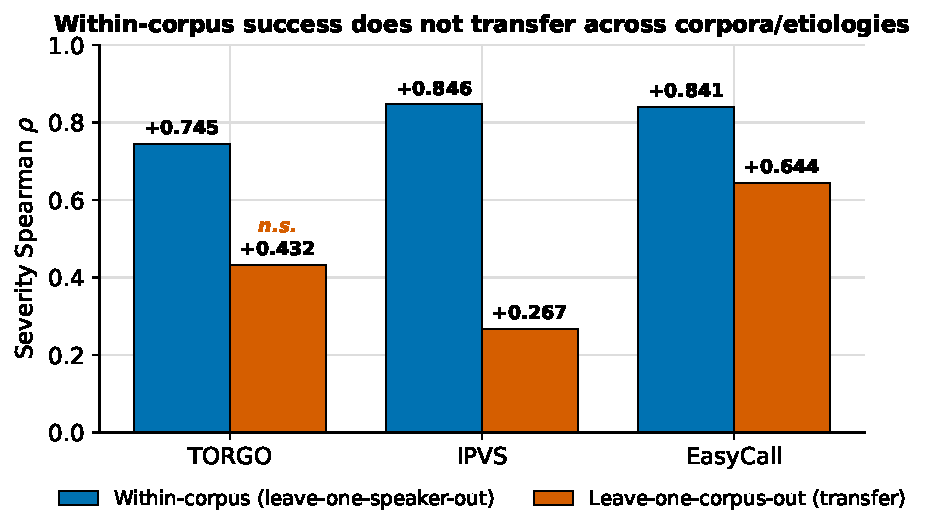
\includegraphics[width=\columnwidth]{fig1_within_vs_loco.pdf}
\caption{Within-corpus severity prediction is strong for all three corpora, but
leave-one-corpus-out transfer degrades and, for the only graded corpus (TORGO),
becomes non-significant.}
\label{fig:xc}
\end{figure}

\subsection{Speaker-identity leakage inflates reference metrics}
Reference-based metrics leak speaker identity when the reference contains the test
speaker's own data. On TORGO a naive per-word reference gives an early-layer
(L1) score of $\rho{=}0.775$; under a strict \emph{leave-one-control-out} (LOCO)
reference it falls to $0.687$---a leakage inflation of
$\Delta{=}\rho_\text{naive}-\rho_\text{LOCO}{=}0.089$. The mid-network layer (L9)
is leakage-robust ($0.756{\to}0.756$, $\Delta{=}0.000$). Early SSL layers encode speaker
identity~\cite{zhu2024wavrx}; we contribute the LOCO reference construction and
quantify the inflation it removes. The layer used for our other results (L9) is
unaffected, so leakage is a hazard specifically for \emph{early-layer} reference
metrics.

\subsection{Pausing and identity confound the ``articulatory'' signal}
Decomposing the reference-distance (ATD) signal by MFA~\cite{mcauliffe2017mfa}
silence/speech alignment: the full metric tracks severity at $\rho{=}0.756$;
\textbf{silence frames alone} reproduce it ($\rho{=}0.775$, $p{<}0.001$);
silence-trimmed speech under a naive reference \emph{collapses}
($\rho{=}0.181$, \ns); but silence-trimmed speech \emph{under a LOCO reference}
\textbf{recovers} ($\rho{=}0.644$, $p{=}0.010$). The honest picture is not ``it is
all silence''---the raw metric conflates articulation, \emph{pausing}, and
\emph{speaker identity}, and only removing both isolates the residual real signal.

\subsection{Cycle-consistency does not predict inversion error}
A natural GT-free reliability metric: invert audio to articulation
(SPARC~\cite{cho2024sparc}), re-synthesise, and measure cycle-consistency in WavLM
space. Tested against \emph{real EMA inversion error} on TORGO controls ($n{=}5$
usable speakers, $22{,}854$ frames, held-out affine alignment, no circularity),
the raw pooled Spearman is $+0.129$ but is a \emph{speech-energy artifact}
($\rho_{\text{faith,energy}}{=}{-}0.468$); the \emph{energy-controlled partial
Spearman} is $-0.001$. A healthy-manifold-centered variant is $+0.39$---the
\emph{wrong sign}. Either way the metric carries no usable information about real
inversion error (Fig.~\ref{fig:cyc}).

\begin{figure}[t]
\centering
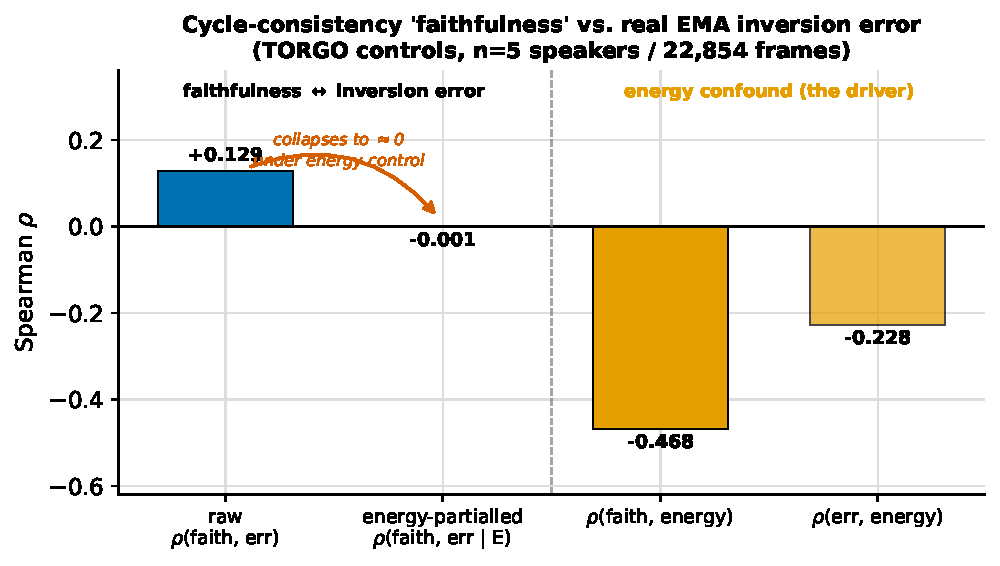
\includegraphics[width=\columnwidth]{fig3_cycle_consistency.pdf}
\caption{The raw faithfulness-versus-error association ($+0.129$) vanishes to
$-0.001$ once speech energy is partialled out, because both faithfulness and
inversion error are themselves driven by energy. Per-frame, TORGO controls,
$n{=}5$ / $22{,}854$ frames.}
\label{fig:cyc}
\end{figure}

\subsection{Inversion is unstable on disordered input}
Kinematic features (tongue range, velocity) derived from SSL inversion do
\emph{not} track the real EMA features (grounding $\rho{=}0.39$, \ns, $n{=}7$). A
``significant'' range-vs-severity correlation ($\rho{=}{+}0.52$, $p{=}0.048$) is in
the clinically \textbf{wrong direction}, consistent with the inverter producing
\emph{more erratic} trajectories on disordered input. Combined with the
$n{\approx}2$ usable dysarthric EMA ceiling, this closes the door on validating
pathological inversion with public data. A downstream articulatory-bottleneck
\emph{clarifier} (encode to the SPARC code, project toward the healthy manifold,
resynthesise) was likewise evaluated honestly and found \emph{null}.

% ===========================================================================
\section{VERITAS-Bench: the Confounds as a Reusable Audit}
% ===========================================================================
The findings above are not one-off observations; they are \emph{validity controls}
any frozen-SSL clinical metric should pass. We package them as VERITAS-Bench: feed
it any per-speaker metric and a corpus and it runs six tests---predictive validity,
speaker-identity leakage (LOCO), silence, energy, cross-corpus transfer, and
representation-level identity AUC---emitting a PASS/WARN/FAIL report card against
documented thresholds.

Applied to our own metrics on TORGO (Table~\ref{tab:bench}) it reproduces every
committed number and, crucially, \emph{discriminates}: the trajectory-distance
metric fails on silence ($24\%$ retained) and identity (AUC $0.996$), whereas a
pooled-embedding probe is silence-robust ($100\%$ retained) yet still fails
cross-corpus transfer and identity. \textbf{No metric passes every control}---which
is the point: a single headline $\rho$ (0.74--0.77 here, all ``PASS'' on predictive
validity) hides the confound a deployment would hit.

\begin{table}[t]
\centering
\caption{VERITAS-Bench report card on TORGO (real, seed 42). Every metric
``passes'' predictive validity yet fails $\ge 1$ confound control.}
\label{tab:bench}
\small
\begin{tabular}{@{}lccc@{}}
\toprule
Control & ATD-L9 & ATD-L1 & Probe\\
\midrule
predictive validity     & PASS $.77$ & PASS $.69$ & PASS $.74$\\
leakage (LOCO $\Delta$) & PASS $.00$ & \textbf{WARN} $.09$ & N/A\\
silence (kept)          & \textbf{FAIL} $24\%$ & --- & WARN $100\%$\\
energy (kept)           & PASS $96\%$ & --- & PASS $80\%$\\
cross-corpus            & \textbf{FAIL} \ns & --- & \textbf{FAIL} \ns\\
identity AUC            & \textbf{FAIL} $.996$ & --- & \textbf{FAIL} $.996$\\
\midrule
\textbf{overall}        & \textbf{FAIL} & \textbf{WARN} & \textbf{FAIL}\\
\bottomrule
\end{tabular}
\end{table}

\begin{figure}[t]
\centering
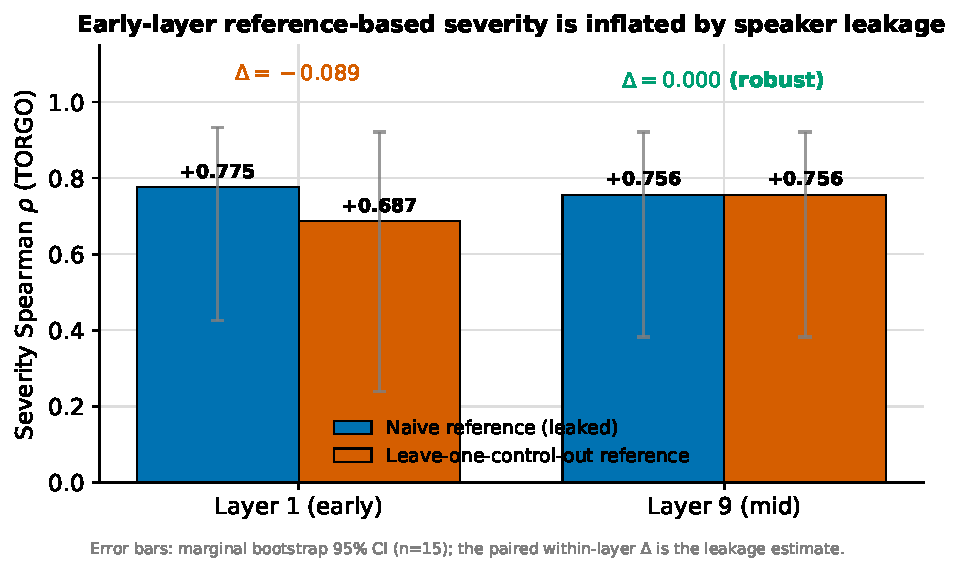
\includegraphics[width=\columnwidth]{fig2_leakage.pdf}
\caption{Reference-based severity on TORGO. From a naive to a leave-one-control-out
reference the early layer (L1) drops by a leakage inflation of
$\Delta{=}\rho_\text{naive}-\rho_\text{LOCO}{=}0.089$, while the mid layer (L9) is
unchanged ($\Delta{=}0.000$).}
\label{fig:leak}
\end{figure}

% ===========================================================================
\section{Recommendations}
% ===========================================================================
For anyone building frozen-SSL clinical-speech metrics:
(1)~\textbf{LOCO references}---never score a speaker against a reference containing
its own data; prefer mid-network layers.
(2)~\textbf{Silence and energy controls}---report VAD-trimmed and energy-partialled
results.
(3)~\textbf{Cross-corpus evaluation}---single-corpus success is not generalisation,
and transfer is metric-dependent.
(4)~\textbf{Ground truth where possible}---validate articulatory claims against real
EMA, and be explicit that pathological EMA barely exists publicly.
(5)~\textbf{Fair, tuned baselines}---a regularised pooled-embedding probe
\emph{ties} trajectory-geometry methods on TORGO (LOSO): the zero-shot
reference-distance score reaches $\rho{=}0.756$ against $0.760$/$0.775$ for
WavLM-L9 mean-pool with Ridge/LinearSVR, and both beat an MFCC baseline
($\rho{=}0.609$).

% ===========================================================================
\section{Conclusion}
% ===========================================================================
Frozen-SSL clinical-speech metrics are easy to build and easy to fool. Across four
metric families and real articulatory ground truth, the apparent signal is
repeatedly \emph{entangled} with a confound---speaker identity, silence/pausing,
energy, or corpus overfitting---and the residual genuine signal, once those are
controlled, is real but \emph{smaller and narrower} than single-corpus numbers
imply. We release the harness, the diagnostics, and VERITAS-Bench so that these
pitfalls are checkable rather than repeated.

\noindent\textbf{Limitations.} $n$ is small for graded severity (TORGO${=}15$;
IPVS/EasyCall are binary detection arms), so the graded cross-corpus result is an
underpowered null rather than a proven absence. All headline numbers map to
committed result files; seed 42; frozen weights; speaker-disjoint splits.

\begin{thebibliography}{00}
\bibitem{chen2022wavlm} S. Chen \emph{et al.}, ``WavLM: Large-scale self-supervised pre-training for full stack speech processing,'' \emph{IEEE J. Sel. Topics Signal Process.}, vol.~16, no.~6, pp.~1505--1518, 2022.
\bibitem{hsu2021hubert} W.-N. Hsu \emph{et al.}, ``HuBERT: Self-supervised speech representation learning by masked prediction of hidden units,'' \emph{IEEE/ACM Trans. Audio, Speech, Language Process.}, vol.~29, pp.~3451--3460, 2021.
\bibitem{rudzicz2012torgo} F. Rudzicz, A. K. Namasivayam, and T. Wolff, ``The TORGO database of acoustic and articulatory speech from speakers with dysarthria,'' \emph{Lang. Resources Eval.}, vol.~46, no.~4, pp.~523--541, 2012.
\bibitem{dimauro2017ipvs} G. Dimauro \emph{et al.}, ``Assessment of speech intelligibility in Parkinson's disease using a speech-to-text system,'' \emph{IEEE Access}, vol.~5, pp.~22199--22208, 2017.
\bibitem{turrisi2021easycall} R. Turrisi \emph{et al.}, ``EasyCall corpus: A dysarthric speech dataset,'' in \emph{Proc. Interspeech}, 2021, pp.~41--45.
\bibitem{frozenssl2026a} B. Muller, A. A. Ortiz Barra\~n\'on, and L. Roberts, ``Training-free cross-lingual dysarthria severity assessment via phonological subspace analysis in self-supervised speech representations,'' \emph{arXiv:2604.10123}, 2026.
\bibitem{frozenssl2026b} B. Muller, A. A. Ortiz Barra\~n\'on, and L. Roberts, ``Phonological subspace collapse is aetiology-specific and cross-lingually stable: Evidence from 3,374 speakers,'' \emph{arXiv:2604.21706}, 2026.
\bibitem{zhu2024wavrx} Y. Zhu and T. H. Falk, ``WavRx: A disease-agnostic, generalizable, and privacy-preserving speech health diagnostic model,'' \emph{arXiv:2406.18731}, 2024.
\bibitem{mcauliffe2017mfa} M. McAuliffe \emph{et al.}, ``Montreal Forced Aligner: Trainable text-speech alignment using Kaldi,'' in \emph{Proc. Interspeech}, 2017, pp.~498--502.
\bibitem{cho2024sparc} C. J. Cho, P. Lee, A. Mohamed, and G. K. Anumanchipalli, ``Coding speech through vocal tract kinematics (SPARC),'' \emph{arXiv:2406.12998}, 2024.
\end{thebibliography}

\end{document}
